\chapter{Detailed comparison of flow models} \label{sec:flow-comparison}
    This appendix follows the results of \S\ref{sec:numerical-methods:blood-flow-experiments} and discusses them in more detail.

    On the 2D placentone simulations presented in Figure \ref{fig:4-models-placentone}, we immediately notice that the flow for S-B in Figure \ref{fig:4-models-placentone:s-b} is the only flow that does not exhibit recirculations in the central cavity. Figures \ref{fig:4-models-placentone:nsb} and \ref{fig:4-models-placentone:ns-nsb} have mostly similar behaviour. To see in which regions of the domains these models differ, we take differences of the solution on the placentone geometry for each combination of model (i.e. for models $i$ and $j$ respectively having velocity fields $\vec{u}_i$ and $\vec{u}_j$, we compute velocity magnitude using the usual Euclidean norm over $\Omega$: $\norm{\vec{u}_i - \vec{u}_j}_{L^2}$). We will refer to these fields as `difference fields'. We study the difference fields only on the placentone geometry, as the differences in flow velocity are mostly localised to the arteries. The difference fields between all three velocity models are presented in Figure \ref{fig:4-models-placentone-norm-log}; note that the difference fields are visualised with a logarithmically-scaled colour scale, so differences may appear exaggerated. The difference fields involving S-B in Figures \ref{fig:4-models-placentone-norm-log:14} and \ref{fig:4-models-placentone-norm-log:12} are relatively large, especially in the central cavity region, but also in the upper section of the diverged artery. The difference field involving NSD with NS-NSD is shown in Figure \ref{fig:4-models-placentone-norm-log:24}, which are clearly similar due to NSD and NS-NSD in themselves behaving similarly. We notice that the difference field in the artery is very small, and in fact small just above the artery, but grows larger further away from the artery mouth. Returning to Figure \ref{fig:4-models-placentone}, we can see the centre of the recirculation zones for NSD sit closer to the artery than those shown for NS-NSD, therefore increasing the value in the difference field in the cavity here; this effect is also likely sensitive to the chosen cavity transition, $\tau$.

    \begin{figure}
        \thisfloatpagestyle{empty}
        % GENERATED WITH MONOLITH COMMIT: XXX
        % GENERATED ON 2024-XX-XX
        \centering
        \begin{subfigure}[b]{0.45\textwidth}
            \centering
            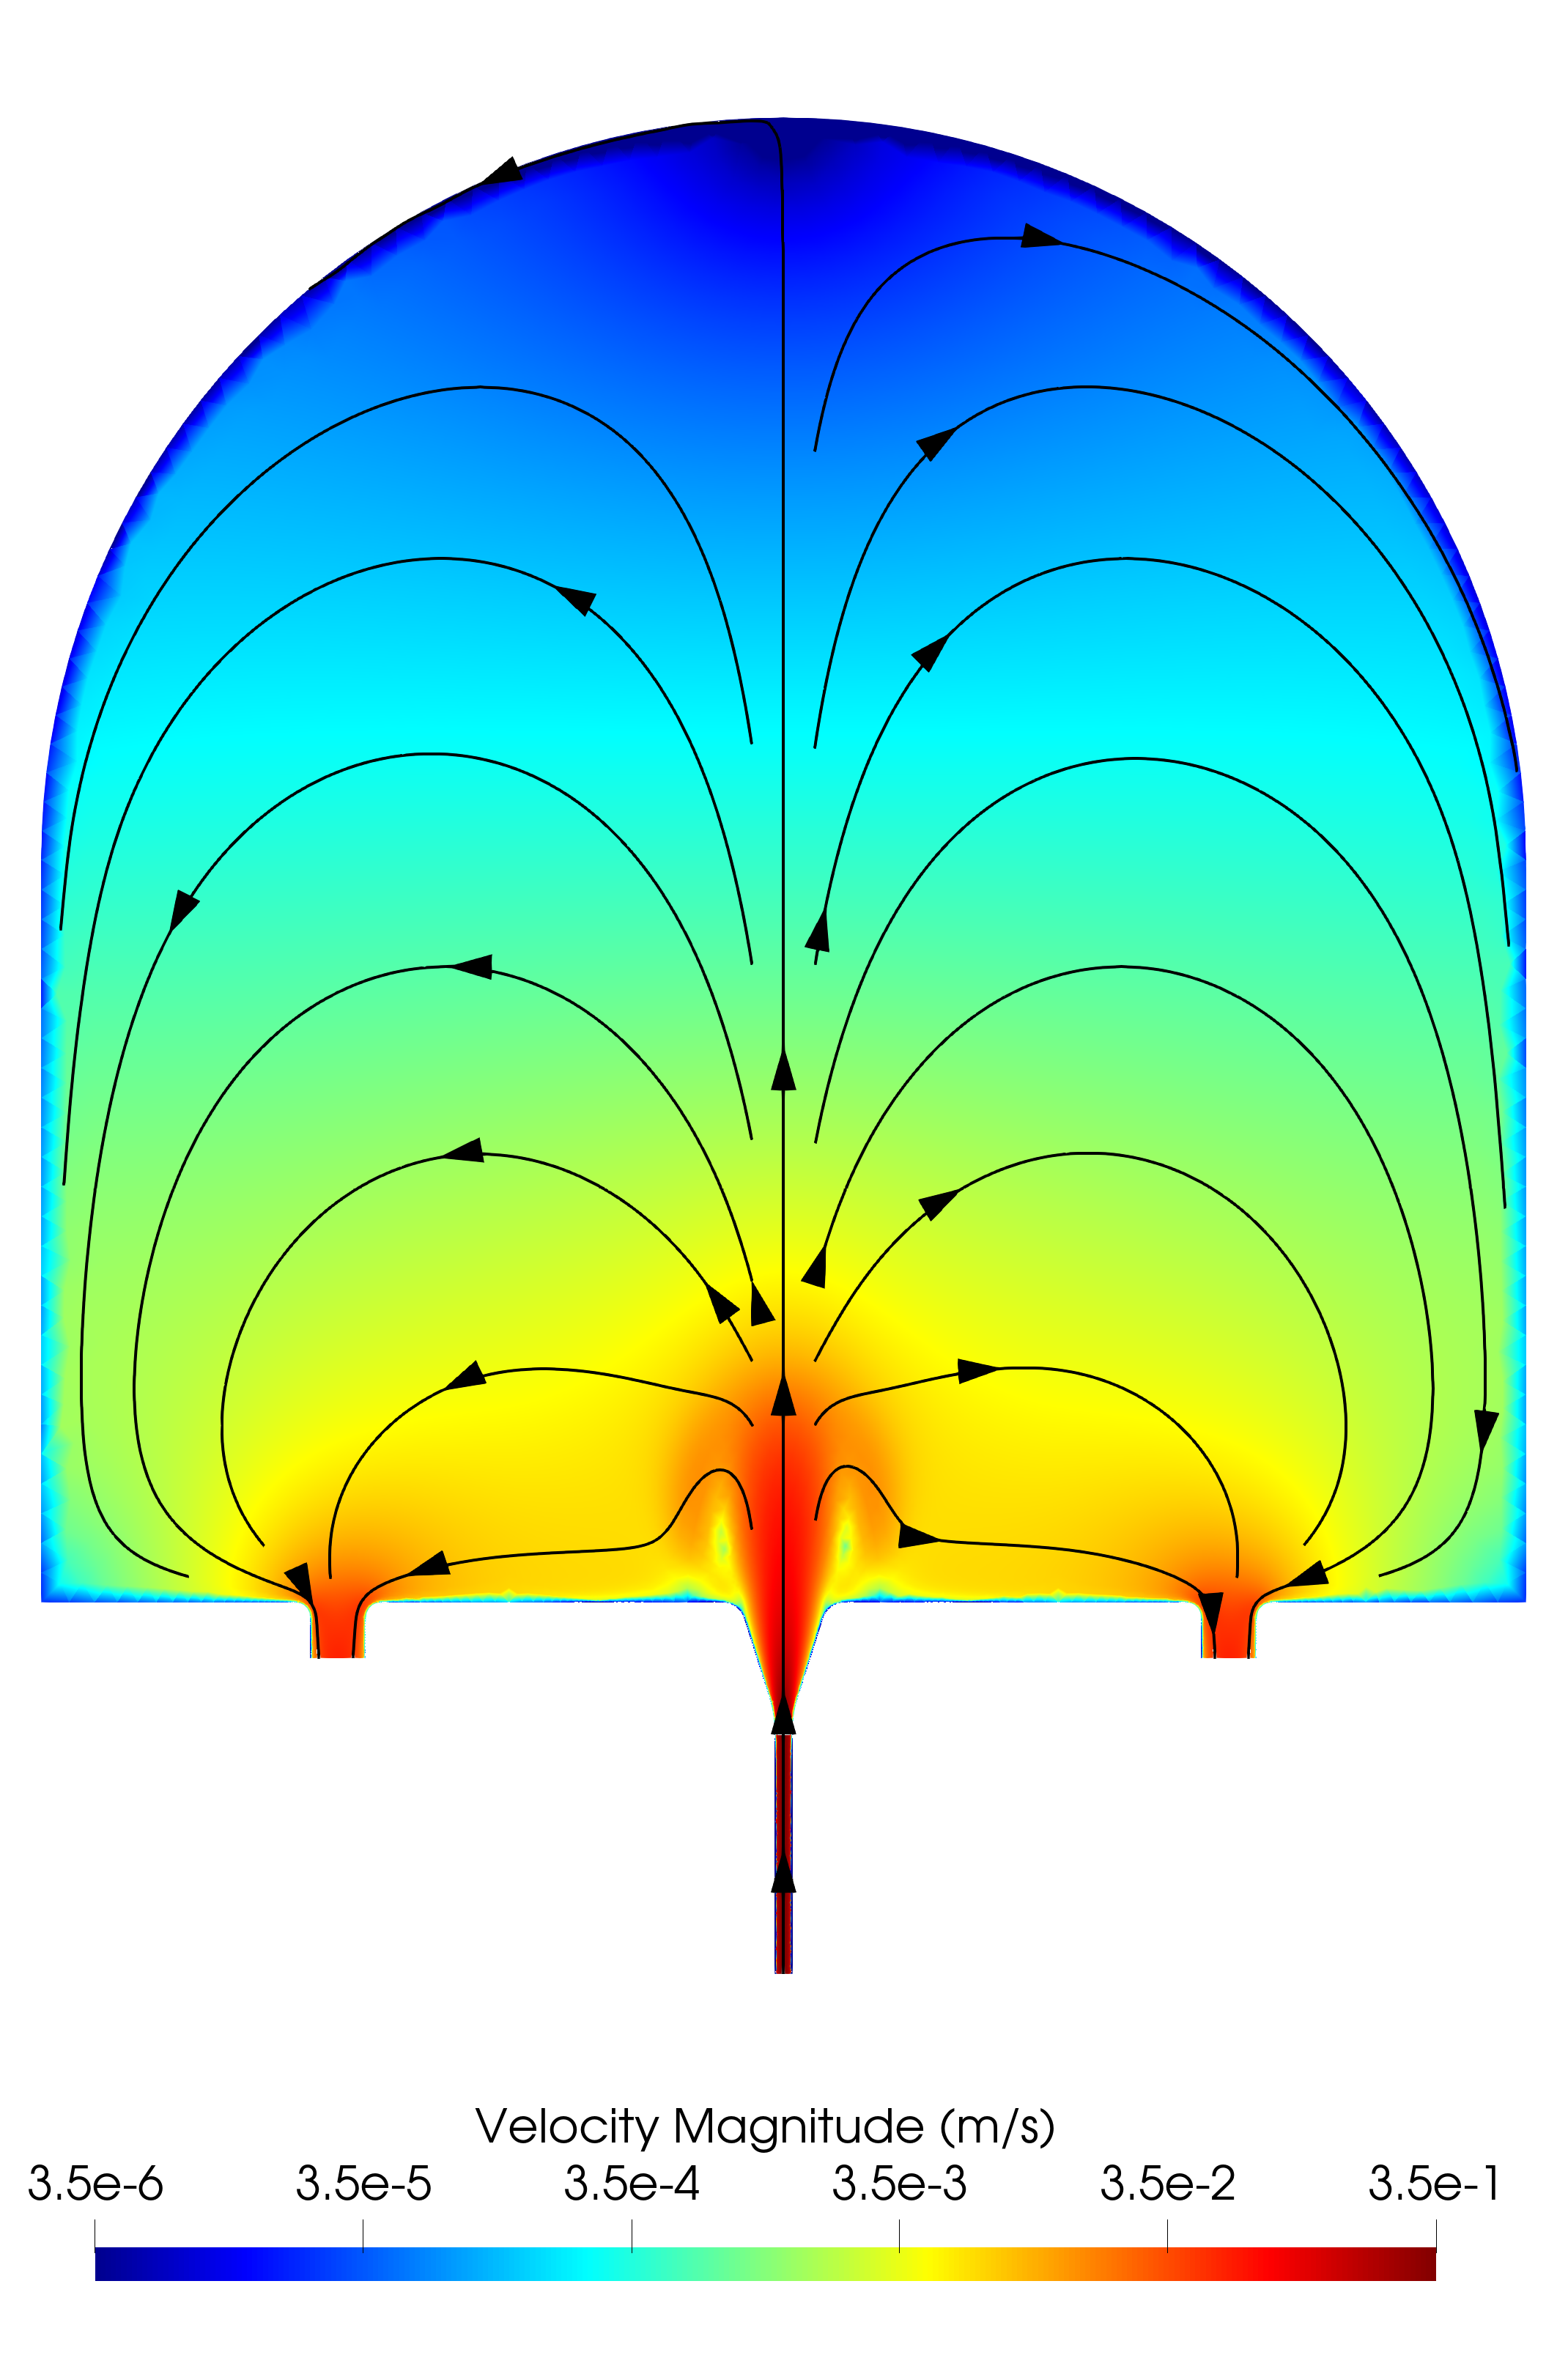
\includegraphics[width=\textwidth]{diagrams/results-modelling/velocity-transport/meshandsoln_dg_velocity_placentone_nsb_velocity-log.png}
            \caption{}
        \end{subfigure}
        \hfill
        \begin{subfigure}[b]{0.45\textwidth}
            \centering
            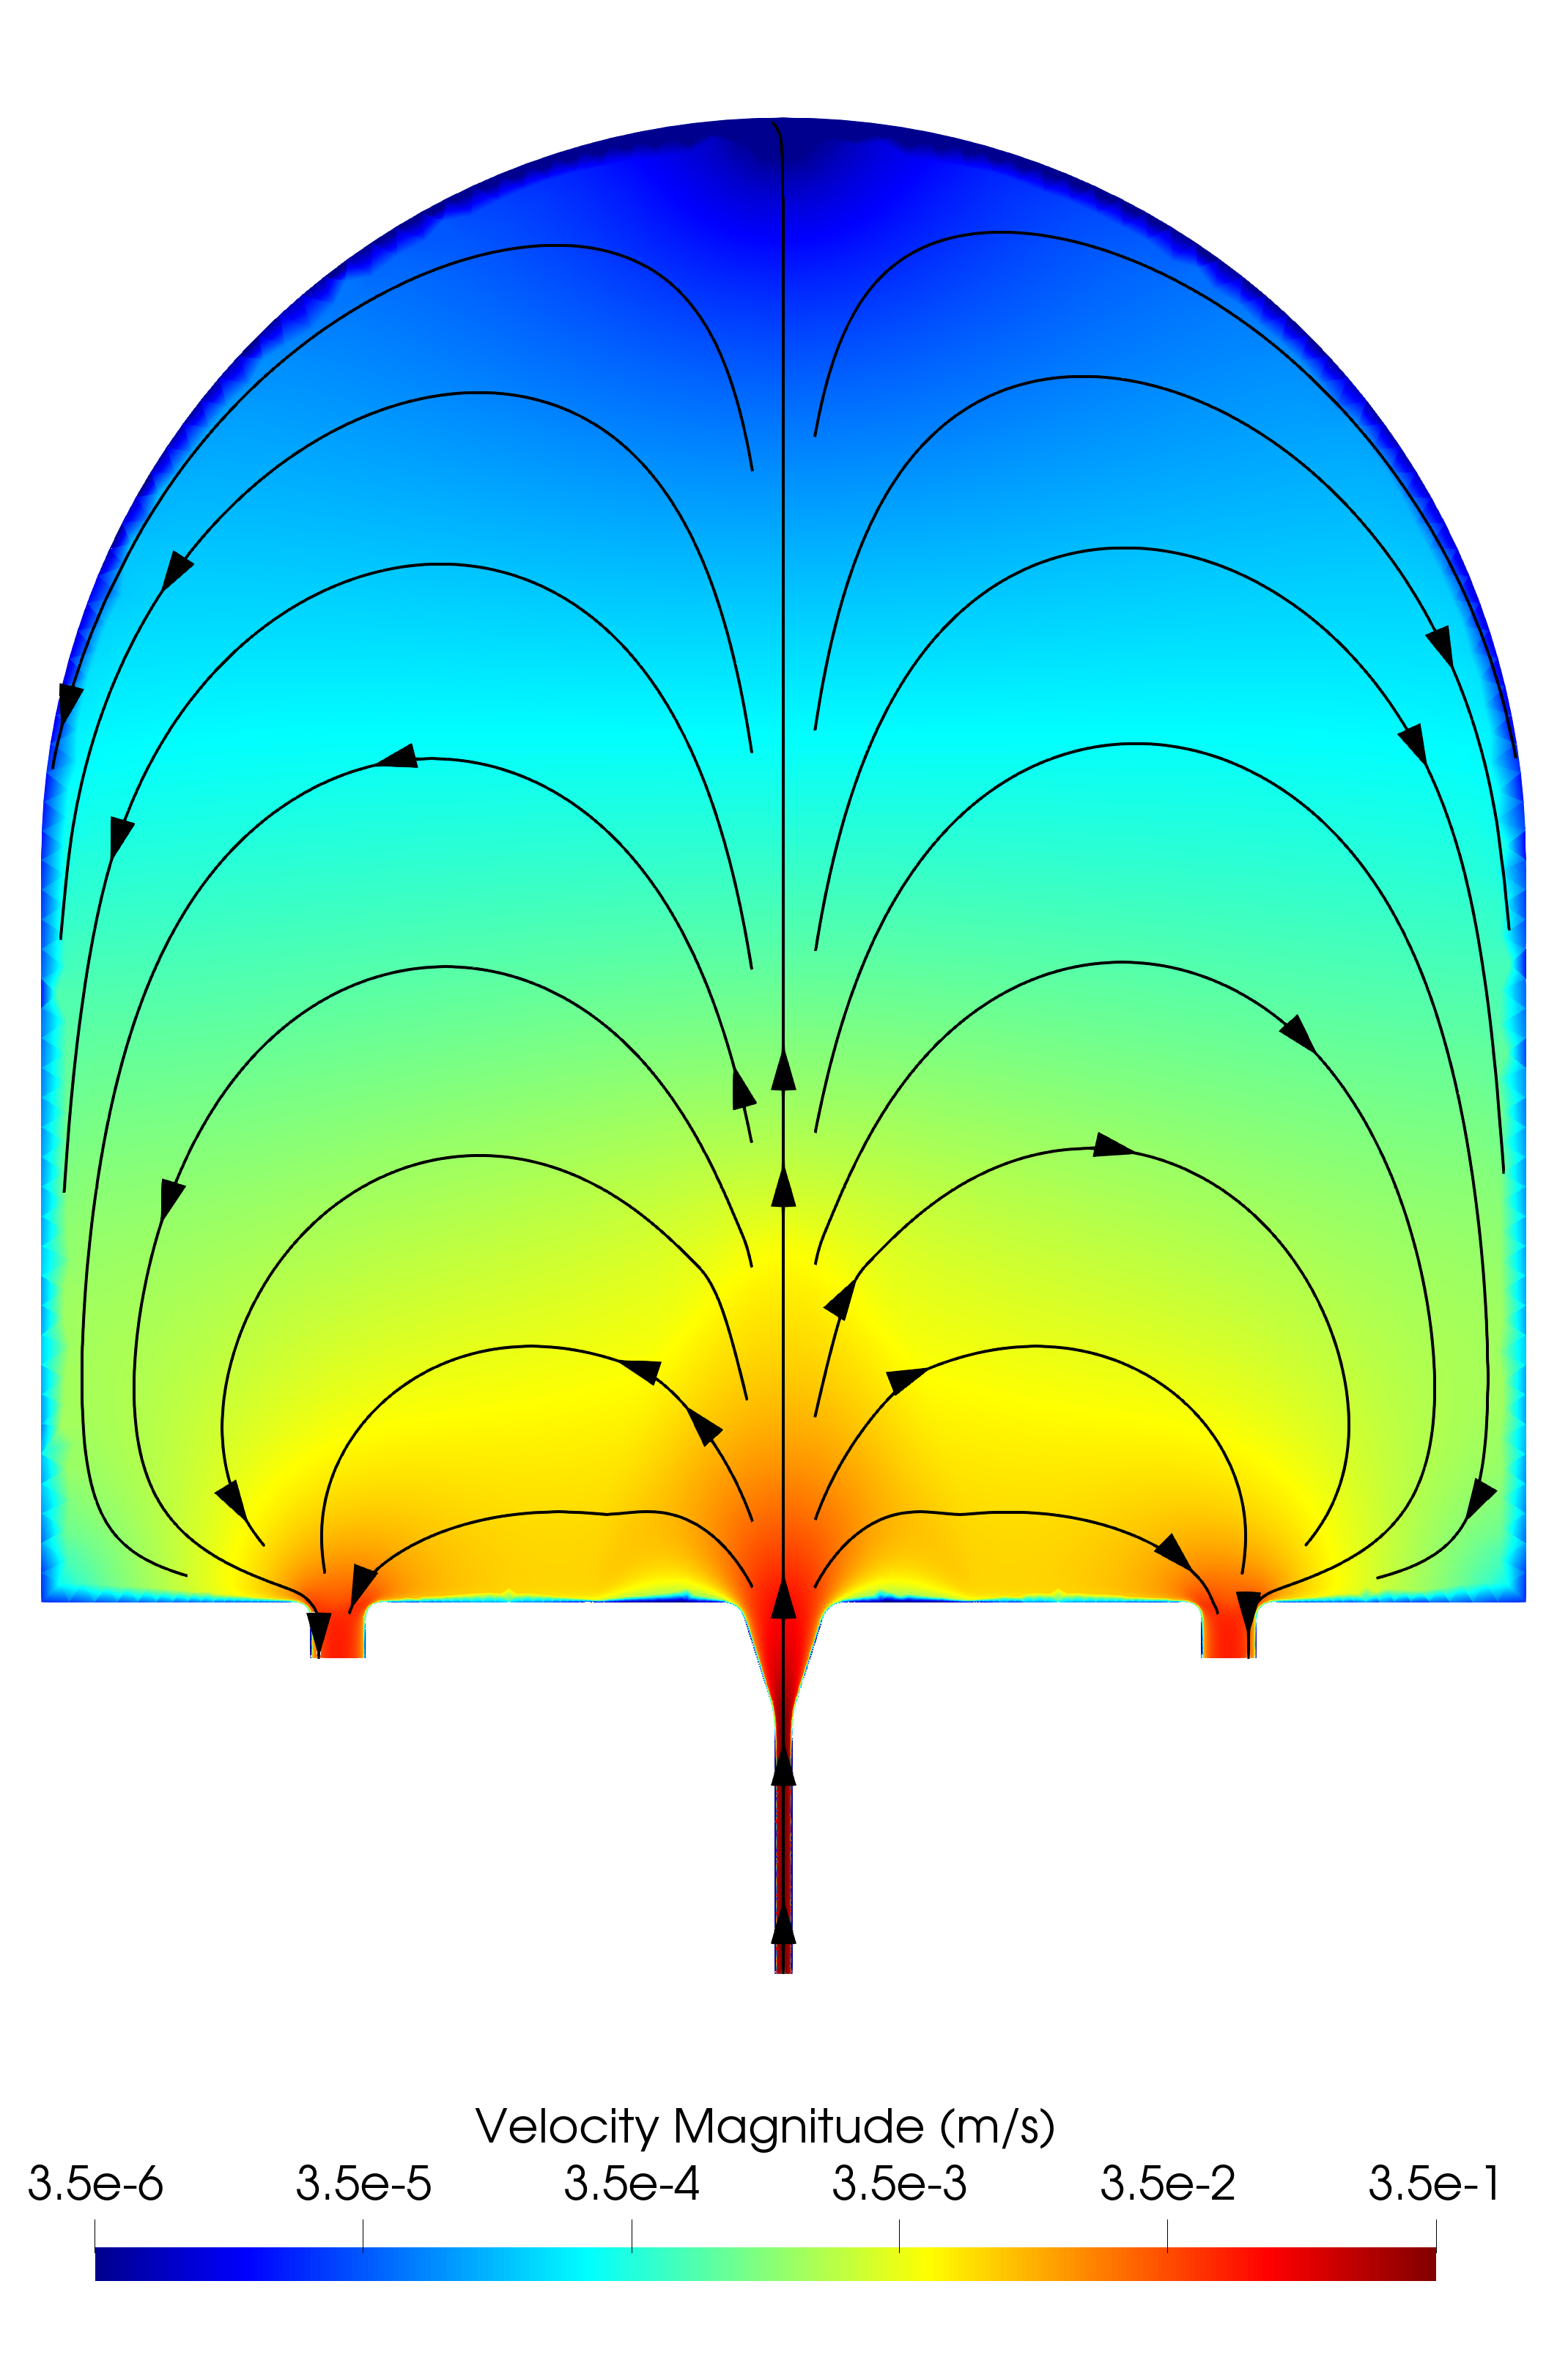
\includegraphics[width=\textwidth]{diagrams/results-modelling/velocity-transport/meshandsoln_dg_velocity_placentone_s-b_velocity-log.png}
            \caption{}
        \end{subfigure}
        \hfill
        \begin{subfigure}[b]{0.45\textwidth}
            \centering
            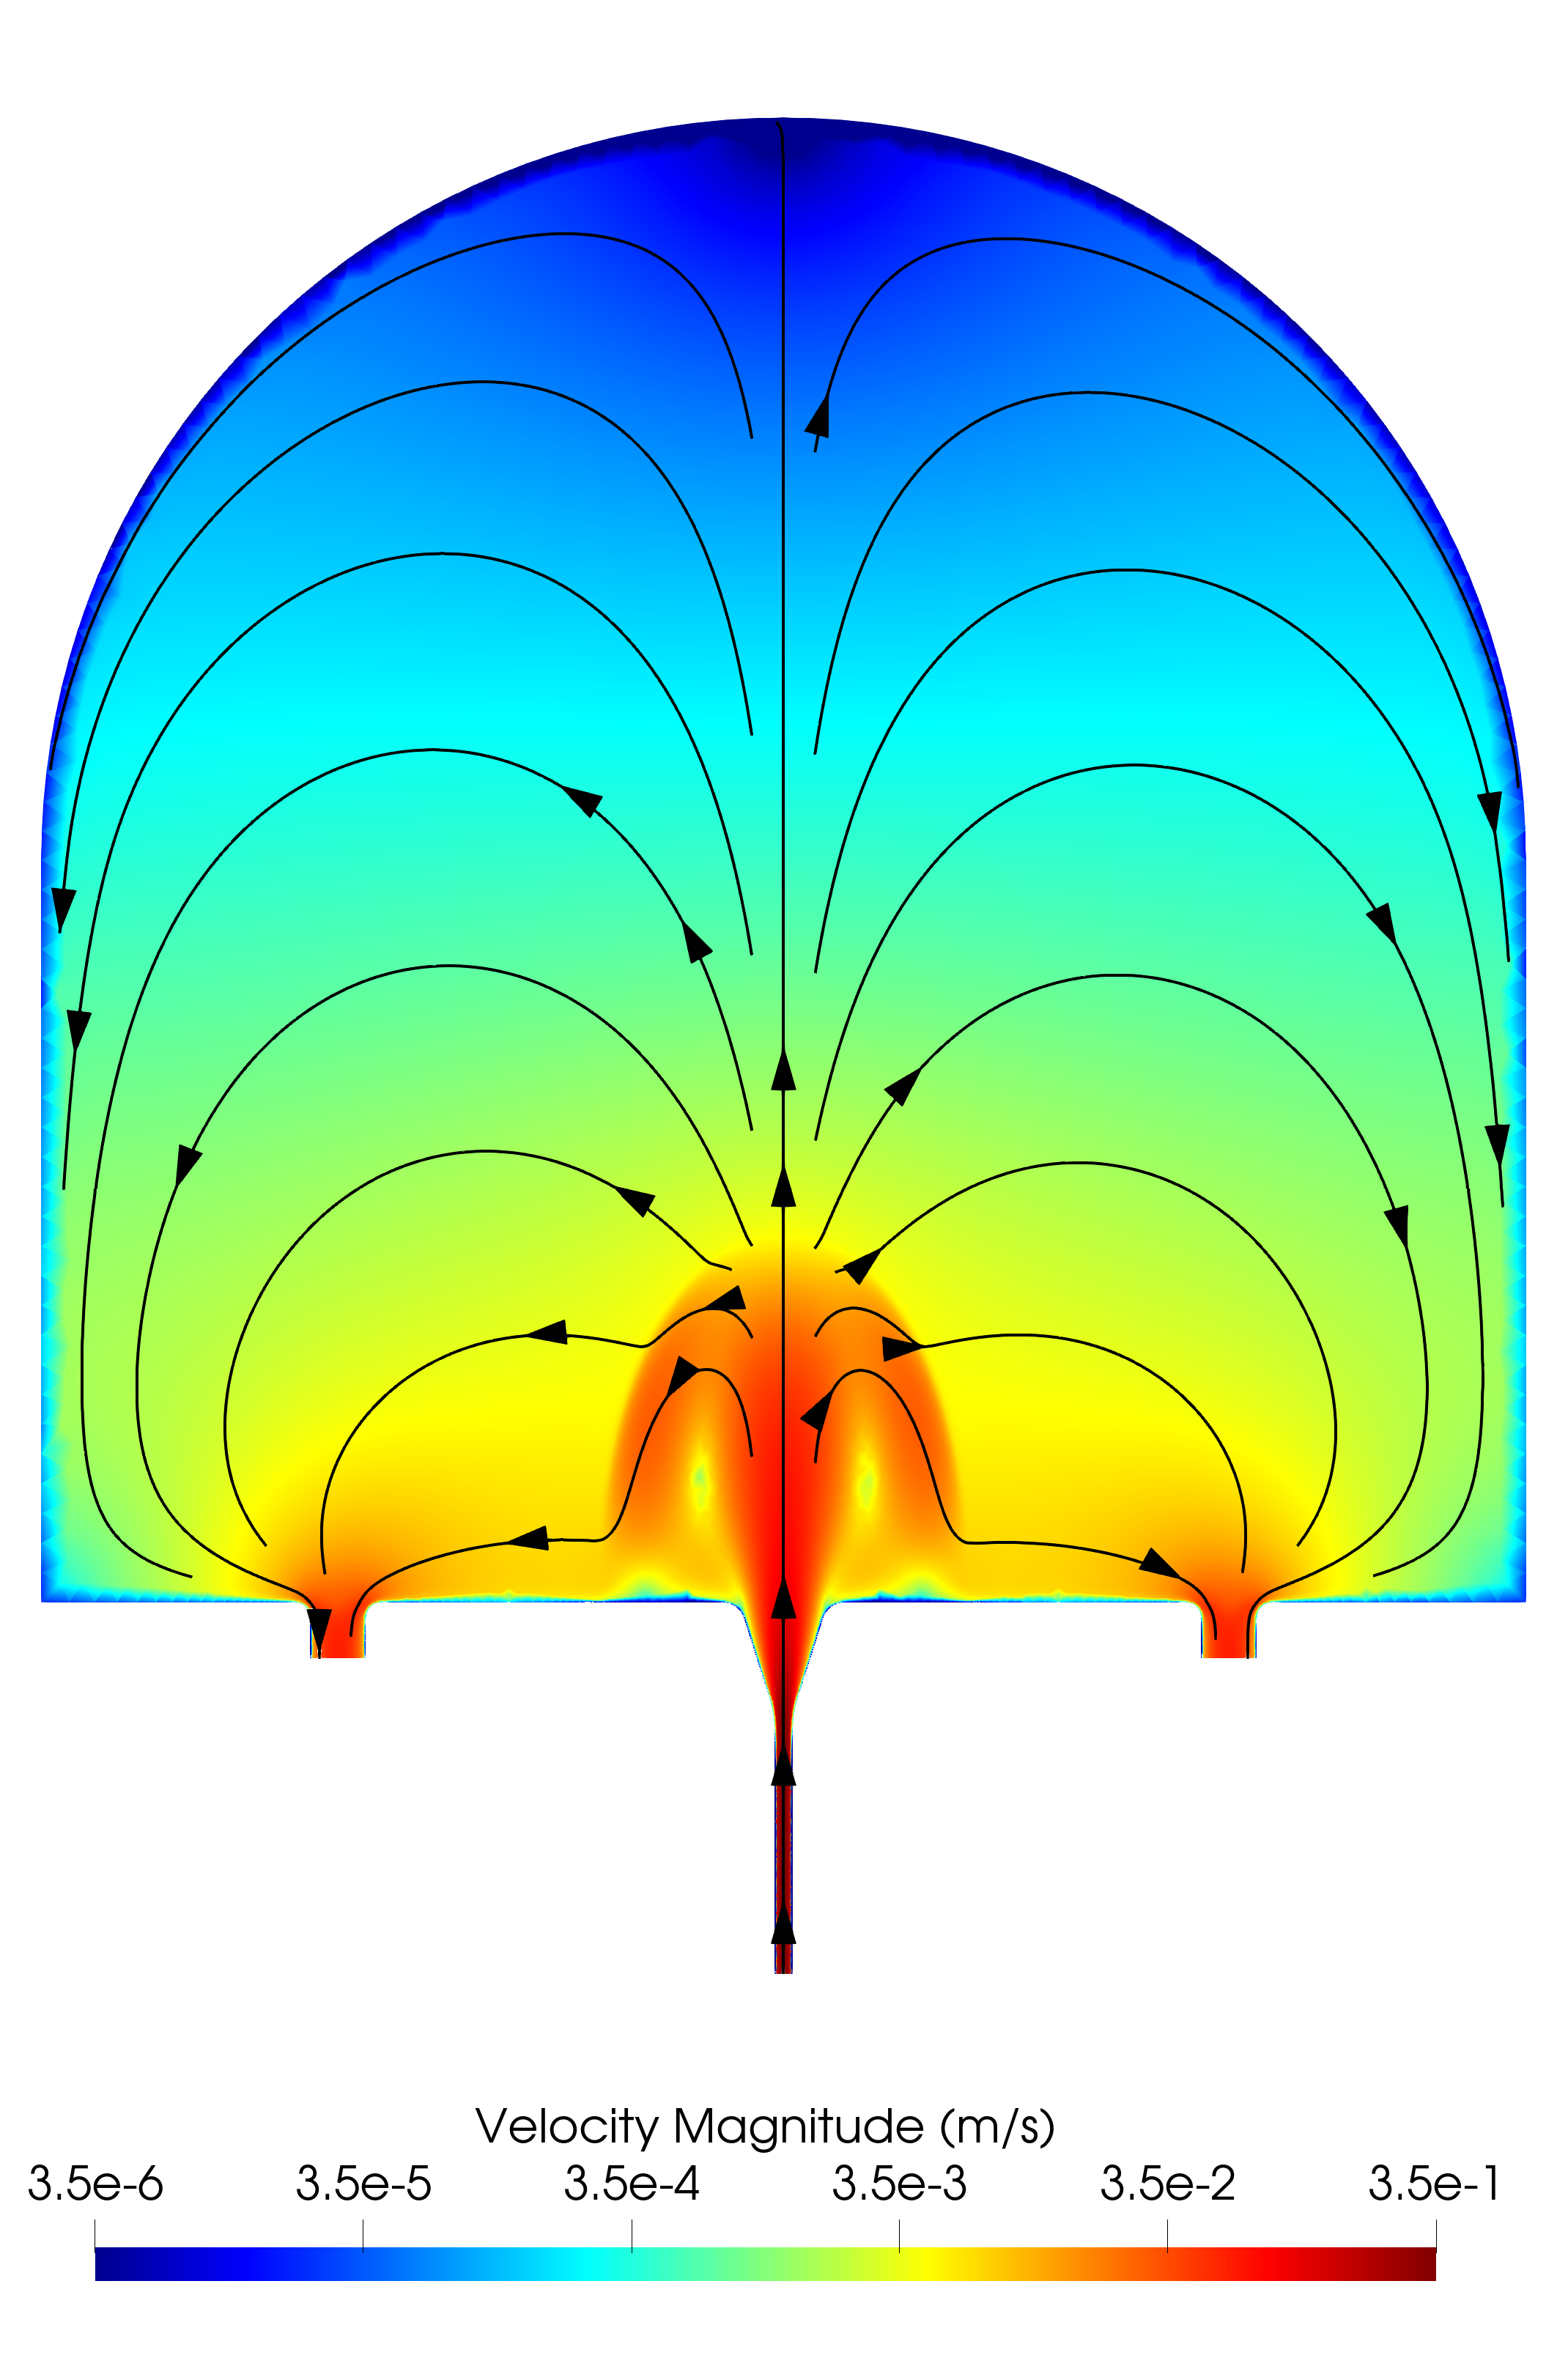
\includegraphics[width=\textwidth]{diagrams/results-modelling/velocity-transport/meshandsoln_dg_velocity_placentone_ns-nsb_velocity-log.png}
            \caption{}
        \end{subfigure}
        \figureretag{fig:4-models-placentone}
        \caption{Velocity plot on placentone geometry (\S\ref{sec:modelling:geometries:2d-placentone}) presenting the results of \S\ref{sec:numerical-methods:blood-flow-experiments:comparison} for the three velocity models: \textbf{NSD} from equation \eqref{eq:nsb}, \textbf{S-B} from equation \eqref{eq:s-b}, and \textbf{NS-NSD} from equation \eqref{eq:ns-nsb}. Plots show a logarithmically-scaled velocity colouring and streamlines shown in black for (a) NSD, (b) S-B, and (c) NS-NSD. All models apply boundary conditions and problem parameters presented in \S\ref{sec:modelling:blood-flow:boundary-conditions}.}
    \end{figure}

    To make a quantitative comparison, we also compute the $L^2$-norm between each combination of solutions. That is to say, for velocity fields $\vec{u}_i$ and $\vec{u}_j$, we compute
    \begin{equation}
        \norm{\vec{u}_i - \vec{u}_j}_{L^2} := \sqrt{\int_\Omega (\vec{u}_i - \vec{u}_j) \cdot (\vec{u}_i - \vec{u}_j) \diff \vec{x}}.
    \end{equation}
    These norms are given in Table \ref{tab:4-models-placentone-l2}. We notice that the largest norm is between S-B and NS-NSD, which likely is contributed to by the lack of recirculations with S-B. This analysis overall shows us quantitatively that all three models are `close' under the $L^2$-norm, and agrees with the qualitative comparisons we made in \S\ref{sec:numerical-methods:blood-flow-experiments:comparison}. 

    \begin{figure}
        % GENERATED WITH MONOLITH COMMIT: XXX
        % GENERATED ON 2024-XX-XX AT XX:XX
        \thisfloatpagestyle{empty}
        \begin{subfigure}[b]{0.45\textwidth}
            \centering
            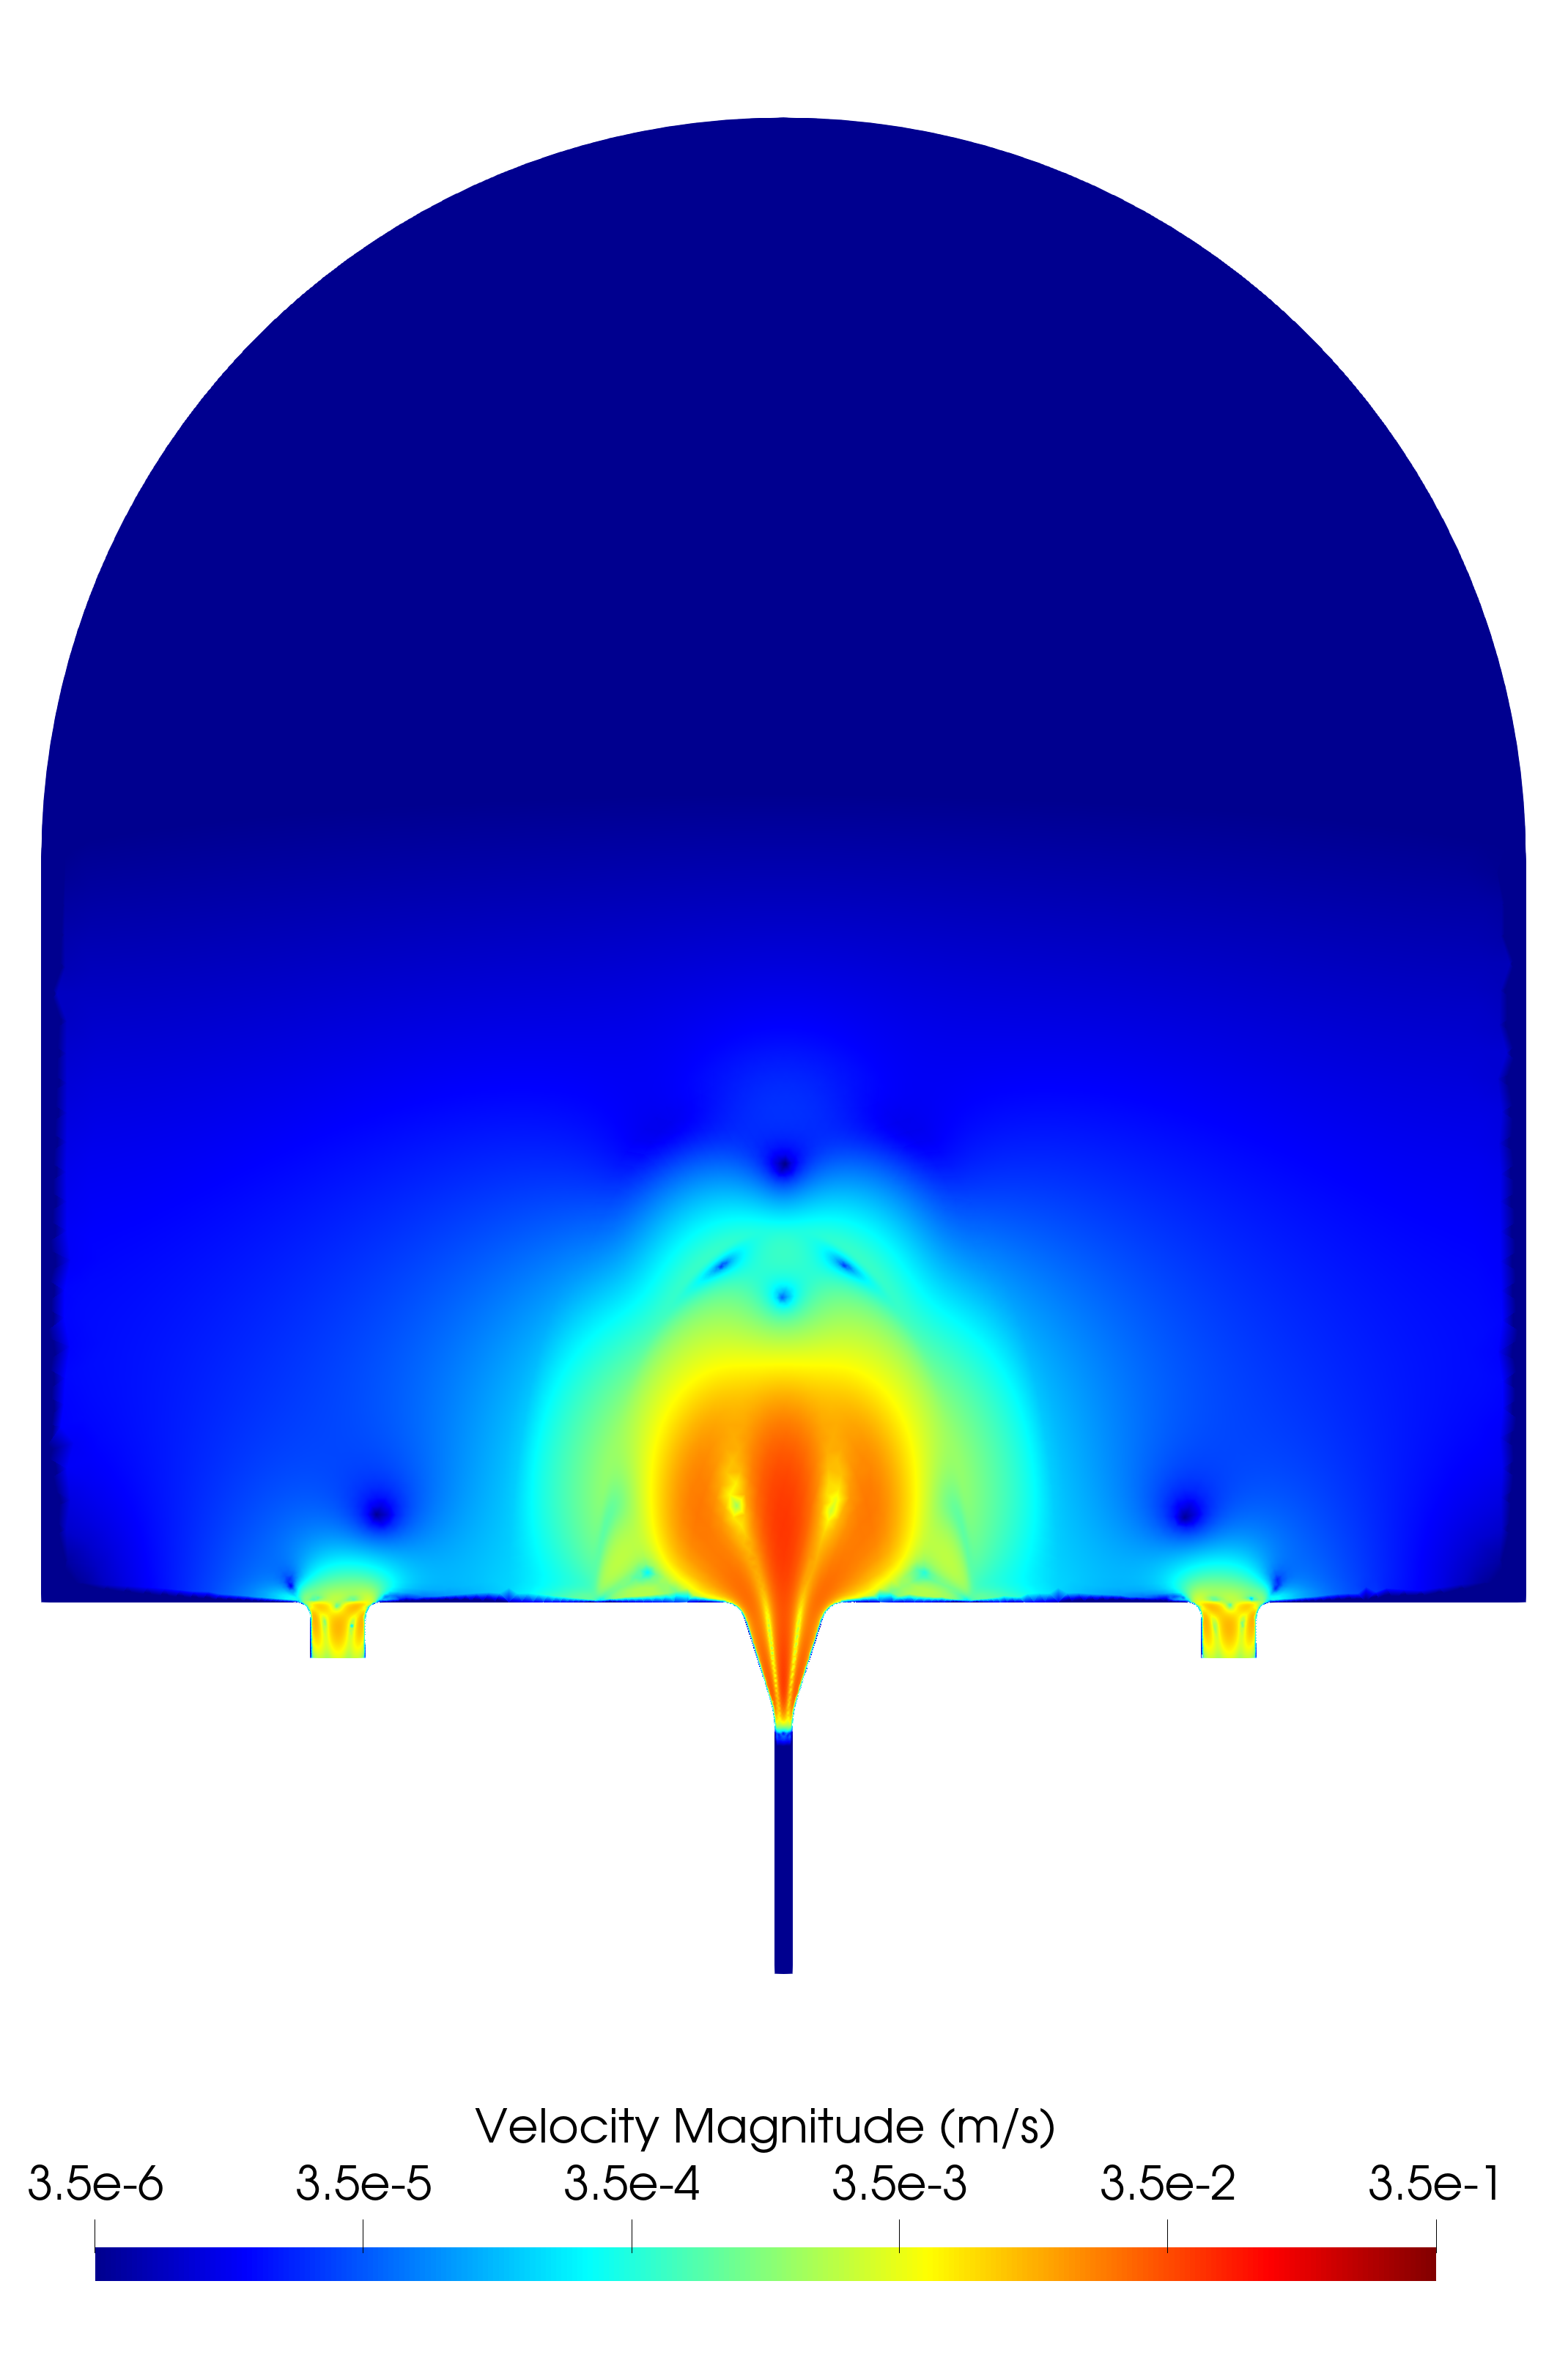
\includegraphics[width=\textwidth]{diagrams/results-modelling/velocity-comparison/meshandsoln_dg_velocity_placentone_14_velocity-log.png}
            \caption{}
            \label{fig:4-models-placentone-norm-log:14}
        \end{subfigure}
        \hfill
        \begin{subfigure}[b]{0.45\textwidth}
            \centering
            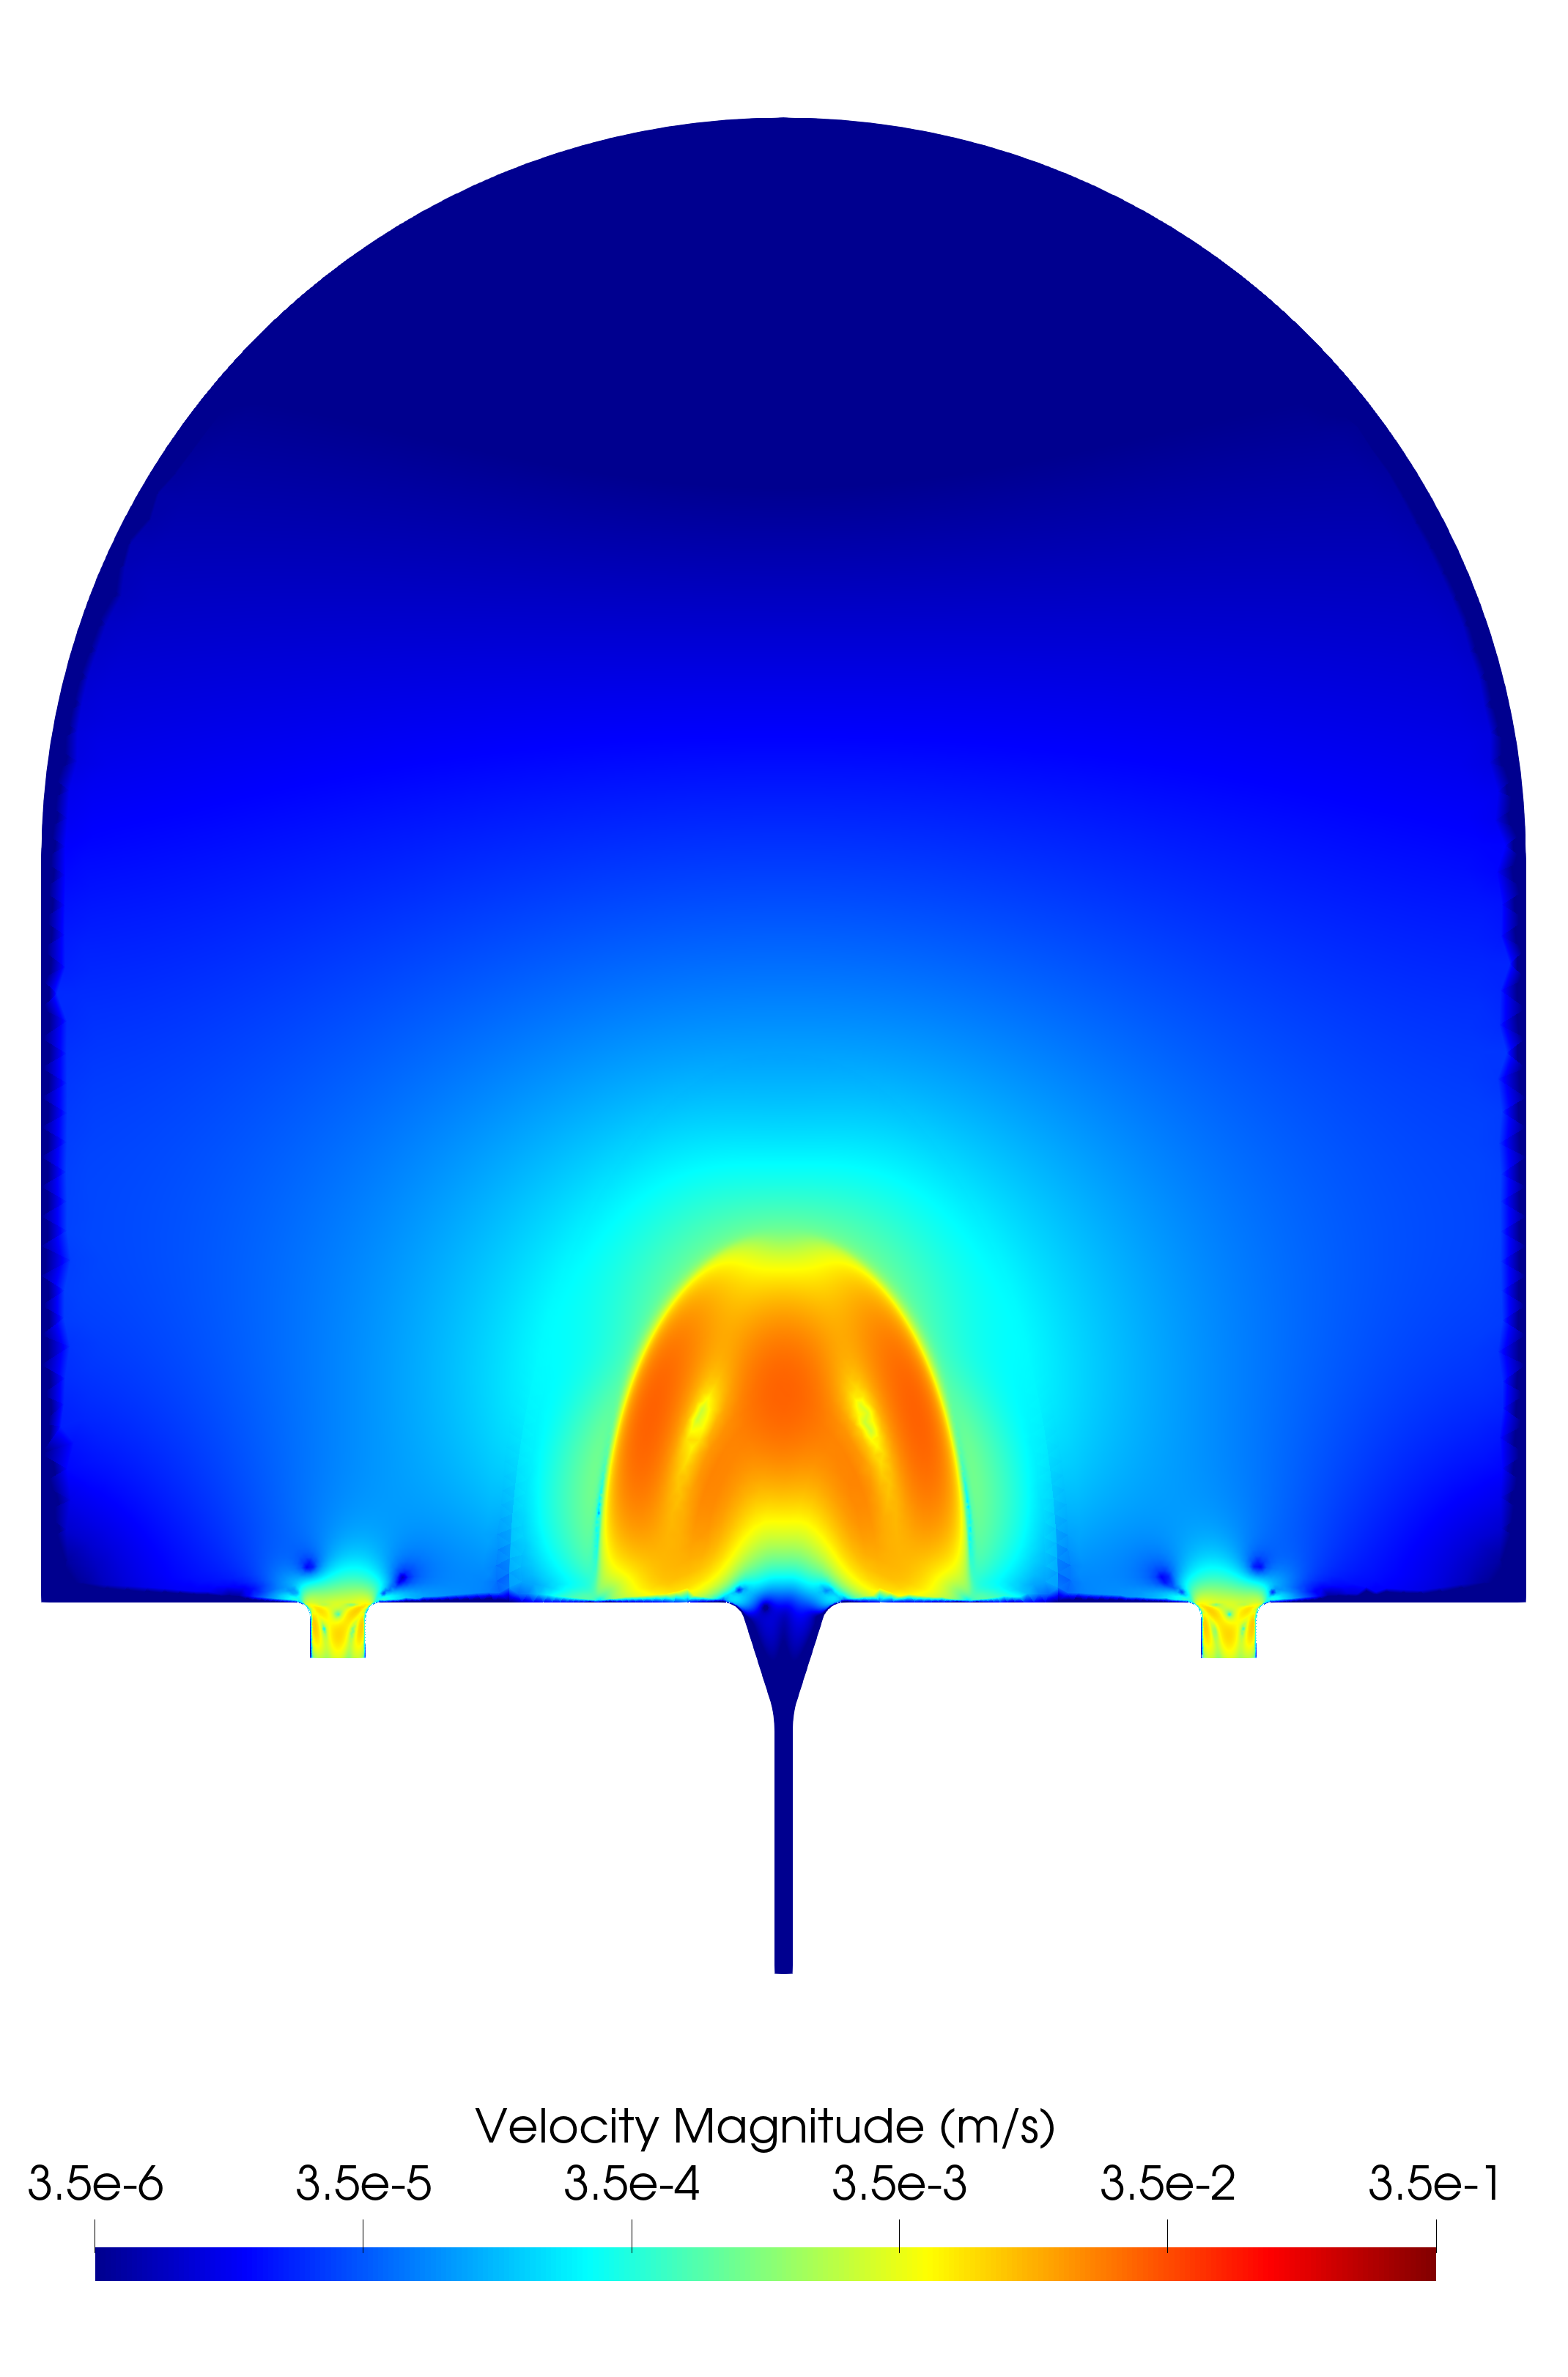
\includegraphics[width=\textwidth]{diagrams/results-modelling/velocity-comparison/meshandsoln_dg_velocity_placentone_24_velocity-log.png}
            \caption{}
            \label{fig:4-models-placentone-norm-log:24}
        \end{subfigure}
        \hfill
        \begin{subfigure}[b]{0.45\textwidth}
            \centering
            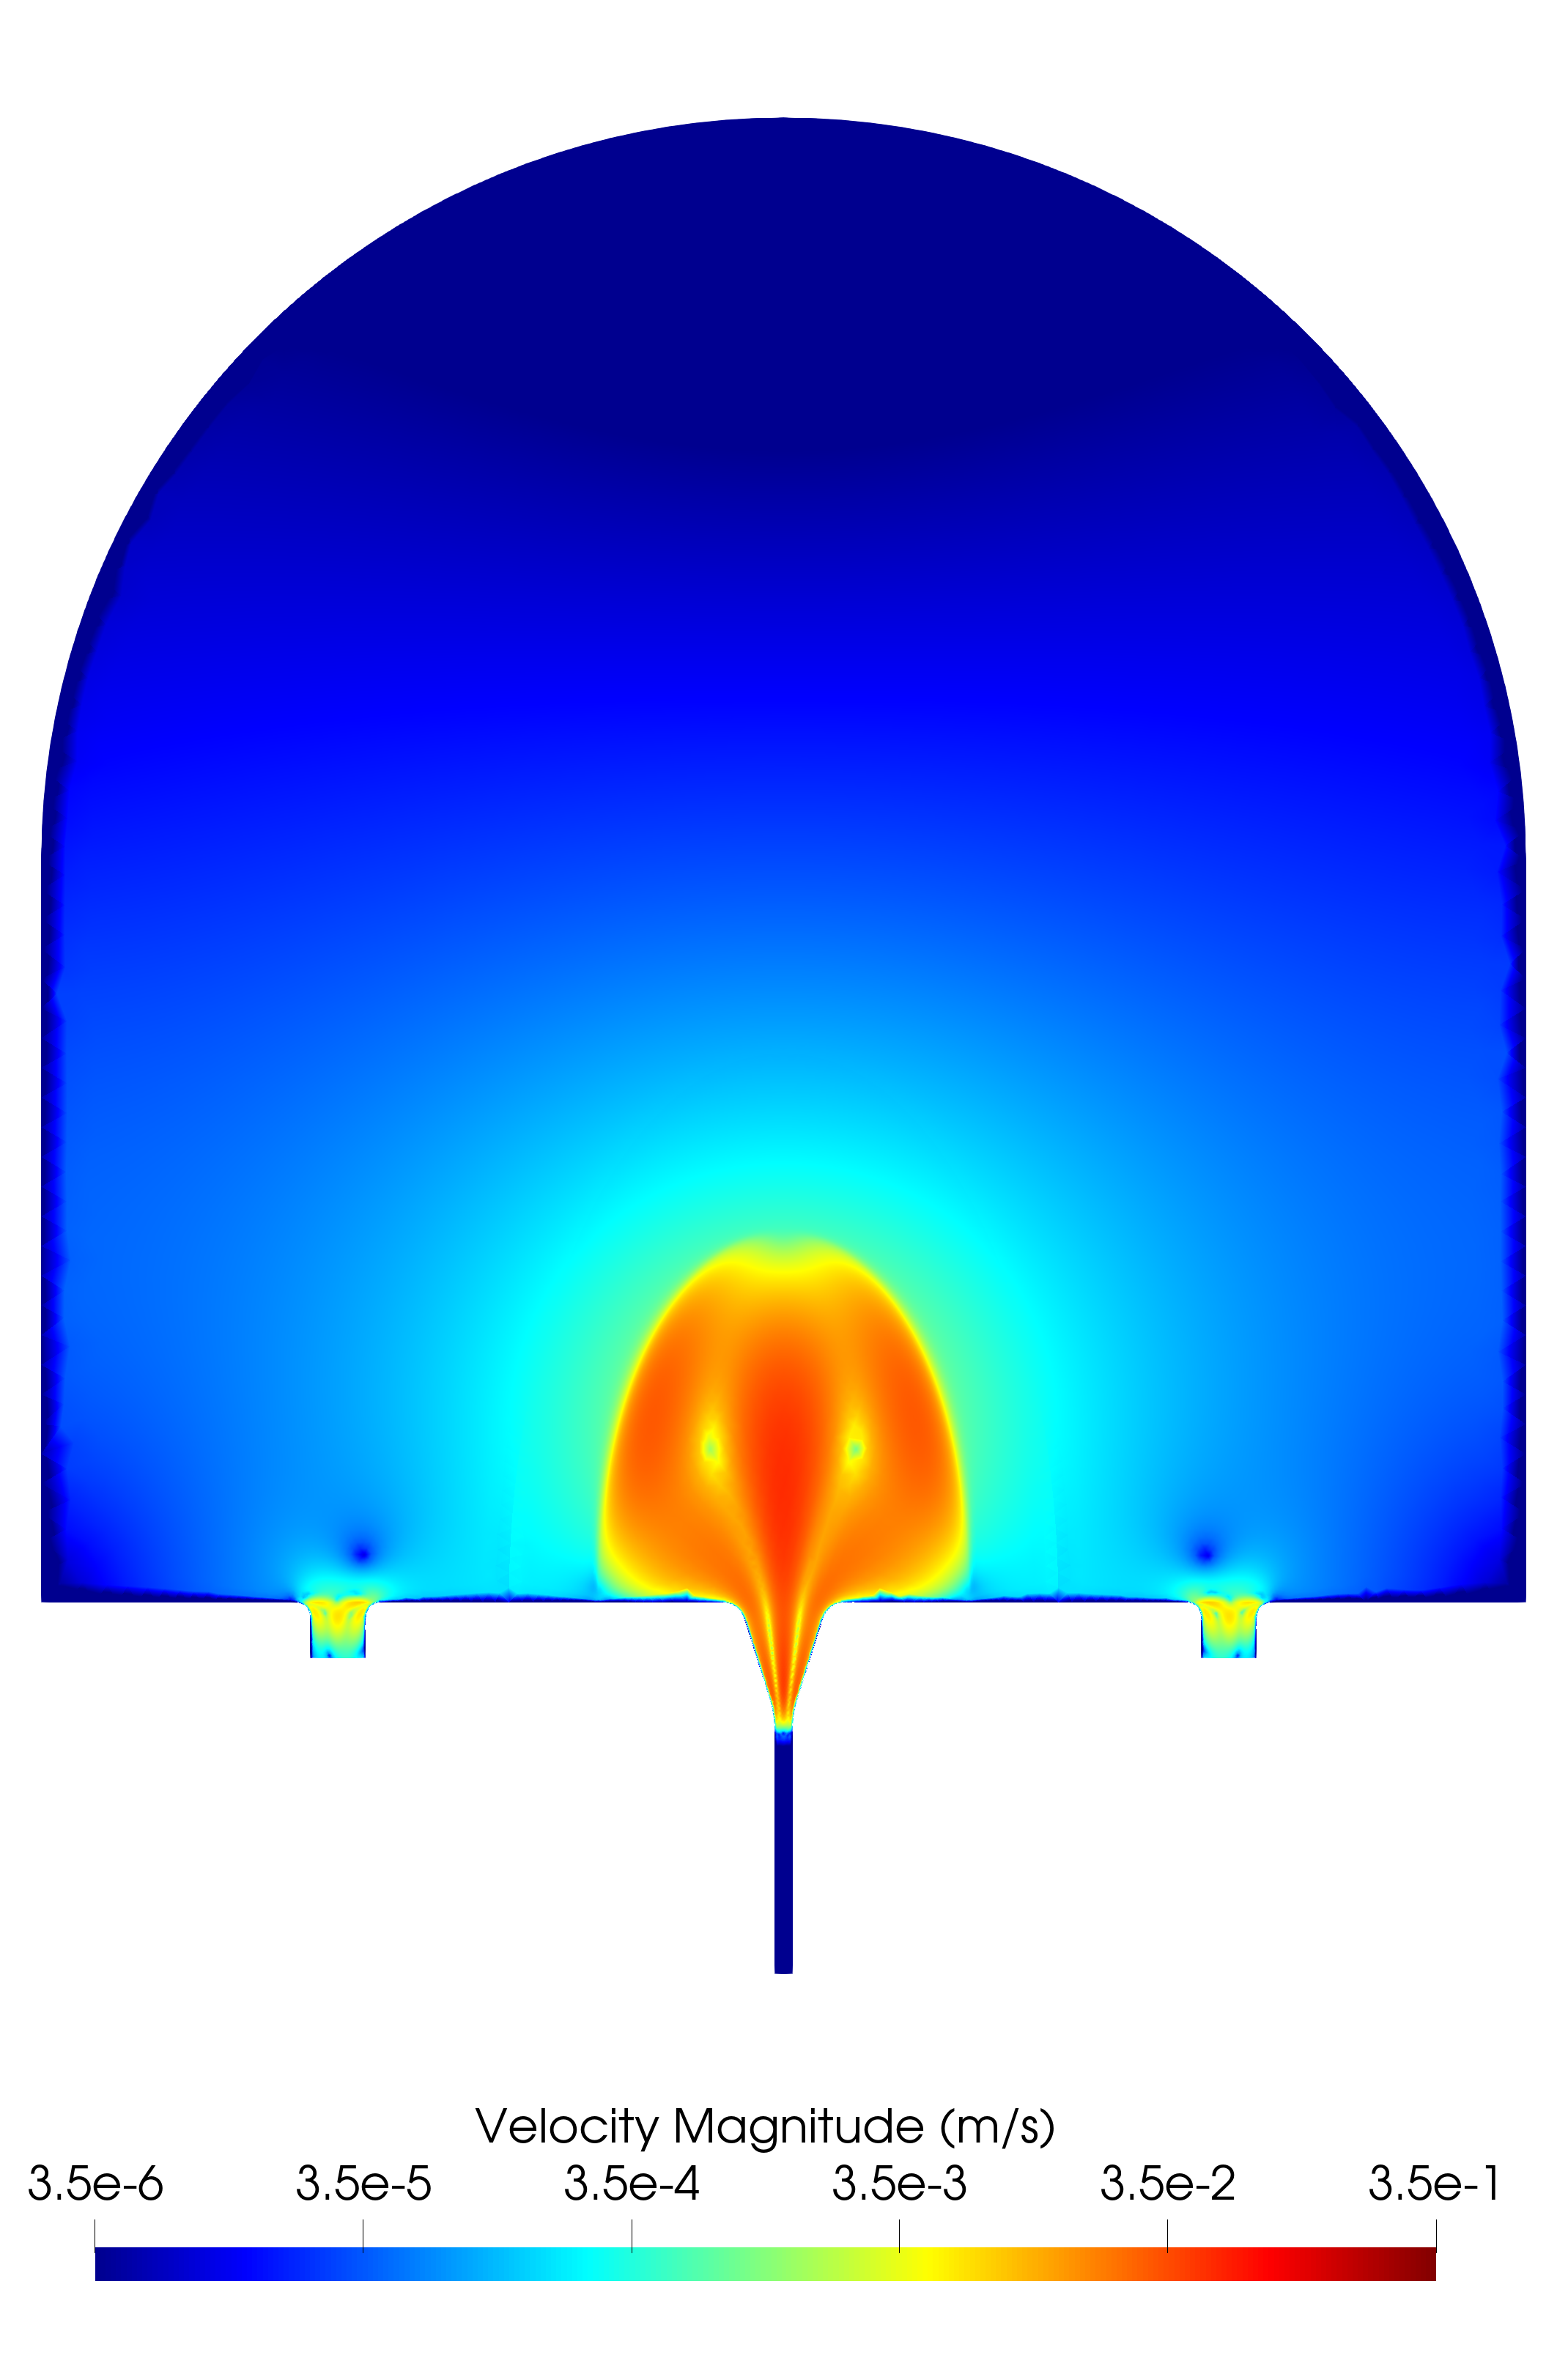
\includegraphics[width=\textwidth]{diagrams/results-modelling/velocity-comparison/meshandsoln_dg_velocity_placentone_12_velocity-log.png}
            \caption{}
            \label{fig:4-models-placentone-norm-log:12}
        \end{subfigure}       

        \caption{Difference fields on a placentone, visualised with a logarithmic colour scaling. Differences are computed between approximations to (a) NSD and S-B (Equations \eqref{eq:nsb} and \eqref{eq:s-b}), (b) NSD and NS-NSD (Equations \eqref{eq:nsb} and \eqref{eq:ns-nsb}), (c) S-B and NS-NSD (Equations \eqref{eq:s-b} and \eqref{eq:ns-nsb}).}
        \label{fig:4-models-placentone-norm-log}
    \end{figure}

    \begin{table}[]
        % GENERATED WITH MONOLITH COMMIT: 0a636bb668309760e0d5884a4fe4684931582d11
        % GENERATED ON 2024-01-12 AT 10:45
        \centering
        \begin{tabular}{c|ccc}
              & NSD & S-B & NS-NSD \\
             \hline
             NSD (Equation \eqref{eq:nsb}) & \num{0} & - & - \\
             S-B (Equation \eqref{eq:s-b}) & \num{8.43E-03} & \num{0} & - \\ 
             NS-NSD (Equation \eqref{eq:ns-nsb}) & \num{8.69E-03} & \num{1.31E-02} & \num{0} 
        \end{tabular}
        \caption{$L_2$-norm of solutions on the placentone geometry using each combination of the three velocity models.}
        \label{tab:4-models-placentone-l2}
    \end{table}